\documentclass[12pt, a4paper]{article}

\title{\textsc{Computer Architecture} Homework 4}
\author{110062219}
\date{\today}

\usepackage{amsmath}
\usepackage{amssymb}
\usepackage{caption}
\usepackage{subcaption}
\usepackage{tikz}
\usepackage{pgfplots}
\usepackage{listings}
\usepackage{float}
\usepackage{tabularx}
\usepackage{makecell}
%\usepackage{geometry}[margin=2cm]

\lstset{
  breaklines=true,
  basicstyle=\ttfamily,
}

\definecolor{nthu}{HTML}{7F1084}

% \renewcommand{\ttdefault}{pcr}

\begin{document}

\maketitle

\tableofcontents

\section{Stuck of Single-Cycle Processor}

\subsection{\texttt{RegWrite}}

\begin{itemize}
\item \texttt{beq}
\item \texttt{sd}
\end{itemize}

\subsection{\texttt{MemRead}}

%\begin{itemize}
%\item \texttt{add}
%\item \texttt{sub}
%\item \texttt{beq}
%\item \texttt{sd}
%\end{itemize}

Though \texttt{MemRead} of all instruction except \texttt{ld} is 0 according to the lecture slide provided by professor, so long as \texttt{MemtoReg} and \texttt{RegWrite} are correct, \texttt{add}, \texttt{sub} and \texttt{beq} would not be affected. Moreover, if our memory supports read and write simultaneously, then \texttt{sd} might still operate correctly.

\subsection{\texttt{ALUOp\textsubscript{1}}}

\begin{itemize}
\item \texttt{sub}
\end{itemize}

The \texttt{ALUOp} of R-type instructions would be \texttt{00} and the ALU would perform addition. Therefore, \texttt{add} is still correct.

\section{Instruction \texttt{0xFF4288E3}}

The instruction represents the assembly \texttt{beq t0,s4,-16}.

\subsection{Values of Signals}

\begin{table}[hbp]
\caption{Values of Control Signals of Branch Instruction}
\label{tab:ctrl}
\centering
\begin{tabular}{ccccccc}
\texttt{Branch} & \texttt{MemRead} & \texttt{MemtoReg} & \texttt{ALUOp} & \texttt{MemWrite} & \texttt{ALUSrc} & \texttt{RegWrite} \\
\hline
1 & 0 & Don't Care & 01 & 0 & 0 & 0
\end{tabular}
\end{table}

\subsection{Inputs of ALU}

Registers \texttt{t0} and \texttt{s4}, i.e., Reg\textsubscript{5} and Reg\textsubscript{20}.

\section{Shortest Possible Clock Time}

The critical path is load instruction: \texttt{PC $\rightarrow$ IM $\rightarrow$ Reg $\rightarrow$ MUX $\rightarrow$ ALU $\rightarrow$ DM $\rightarrow$ MUX $\rightarrow$ Reg}. Since we're writing back to register, we should delay for setup time. Thus the shortest possible clock time is $30+200+140+30+160+200+30+20=810$ps.

\section{Structural Hazard}

\subsection{Stalls}

Before we fetch an instruction, we first check that whether \texttt{MemRead}, \texttt{MemWrite} in \texttt{EX/MEM} pipeline register is set or not, i.e., the instruction in \texttt{MEM} stage is \texttt{ld} or \texttt{sd}. If so, then we have to stall and not to fetch the instruction.

Notwithstanding, suppose that our memory supports read and write simultaneously, then even though \texttt{MemWrite} in \texttt{EX/MEM} pipeline register is set, we're still able to fetch the incoming instruction. So in this case, we only have to stop if the instruction in \texttt{MEM} stage is \texttt{ld}.

\begin{figure}[htbp]
\centering
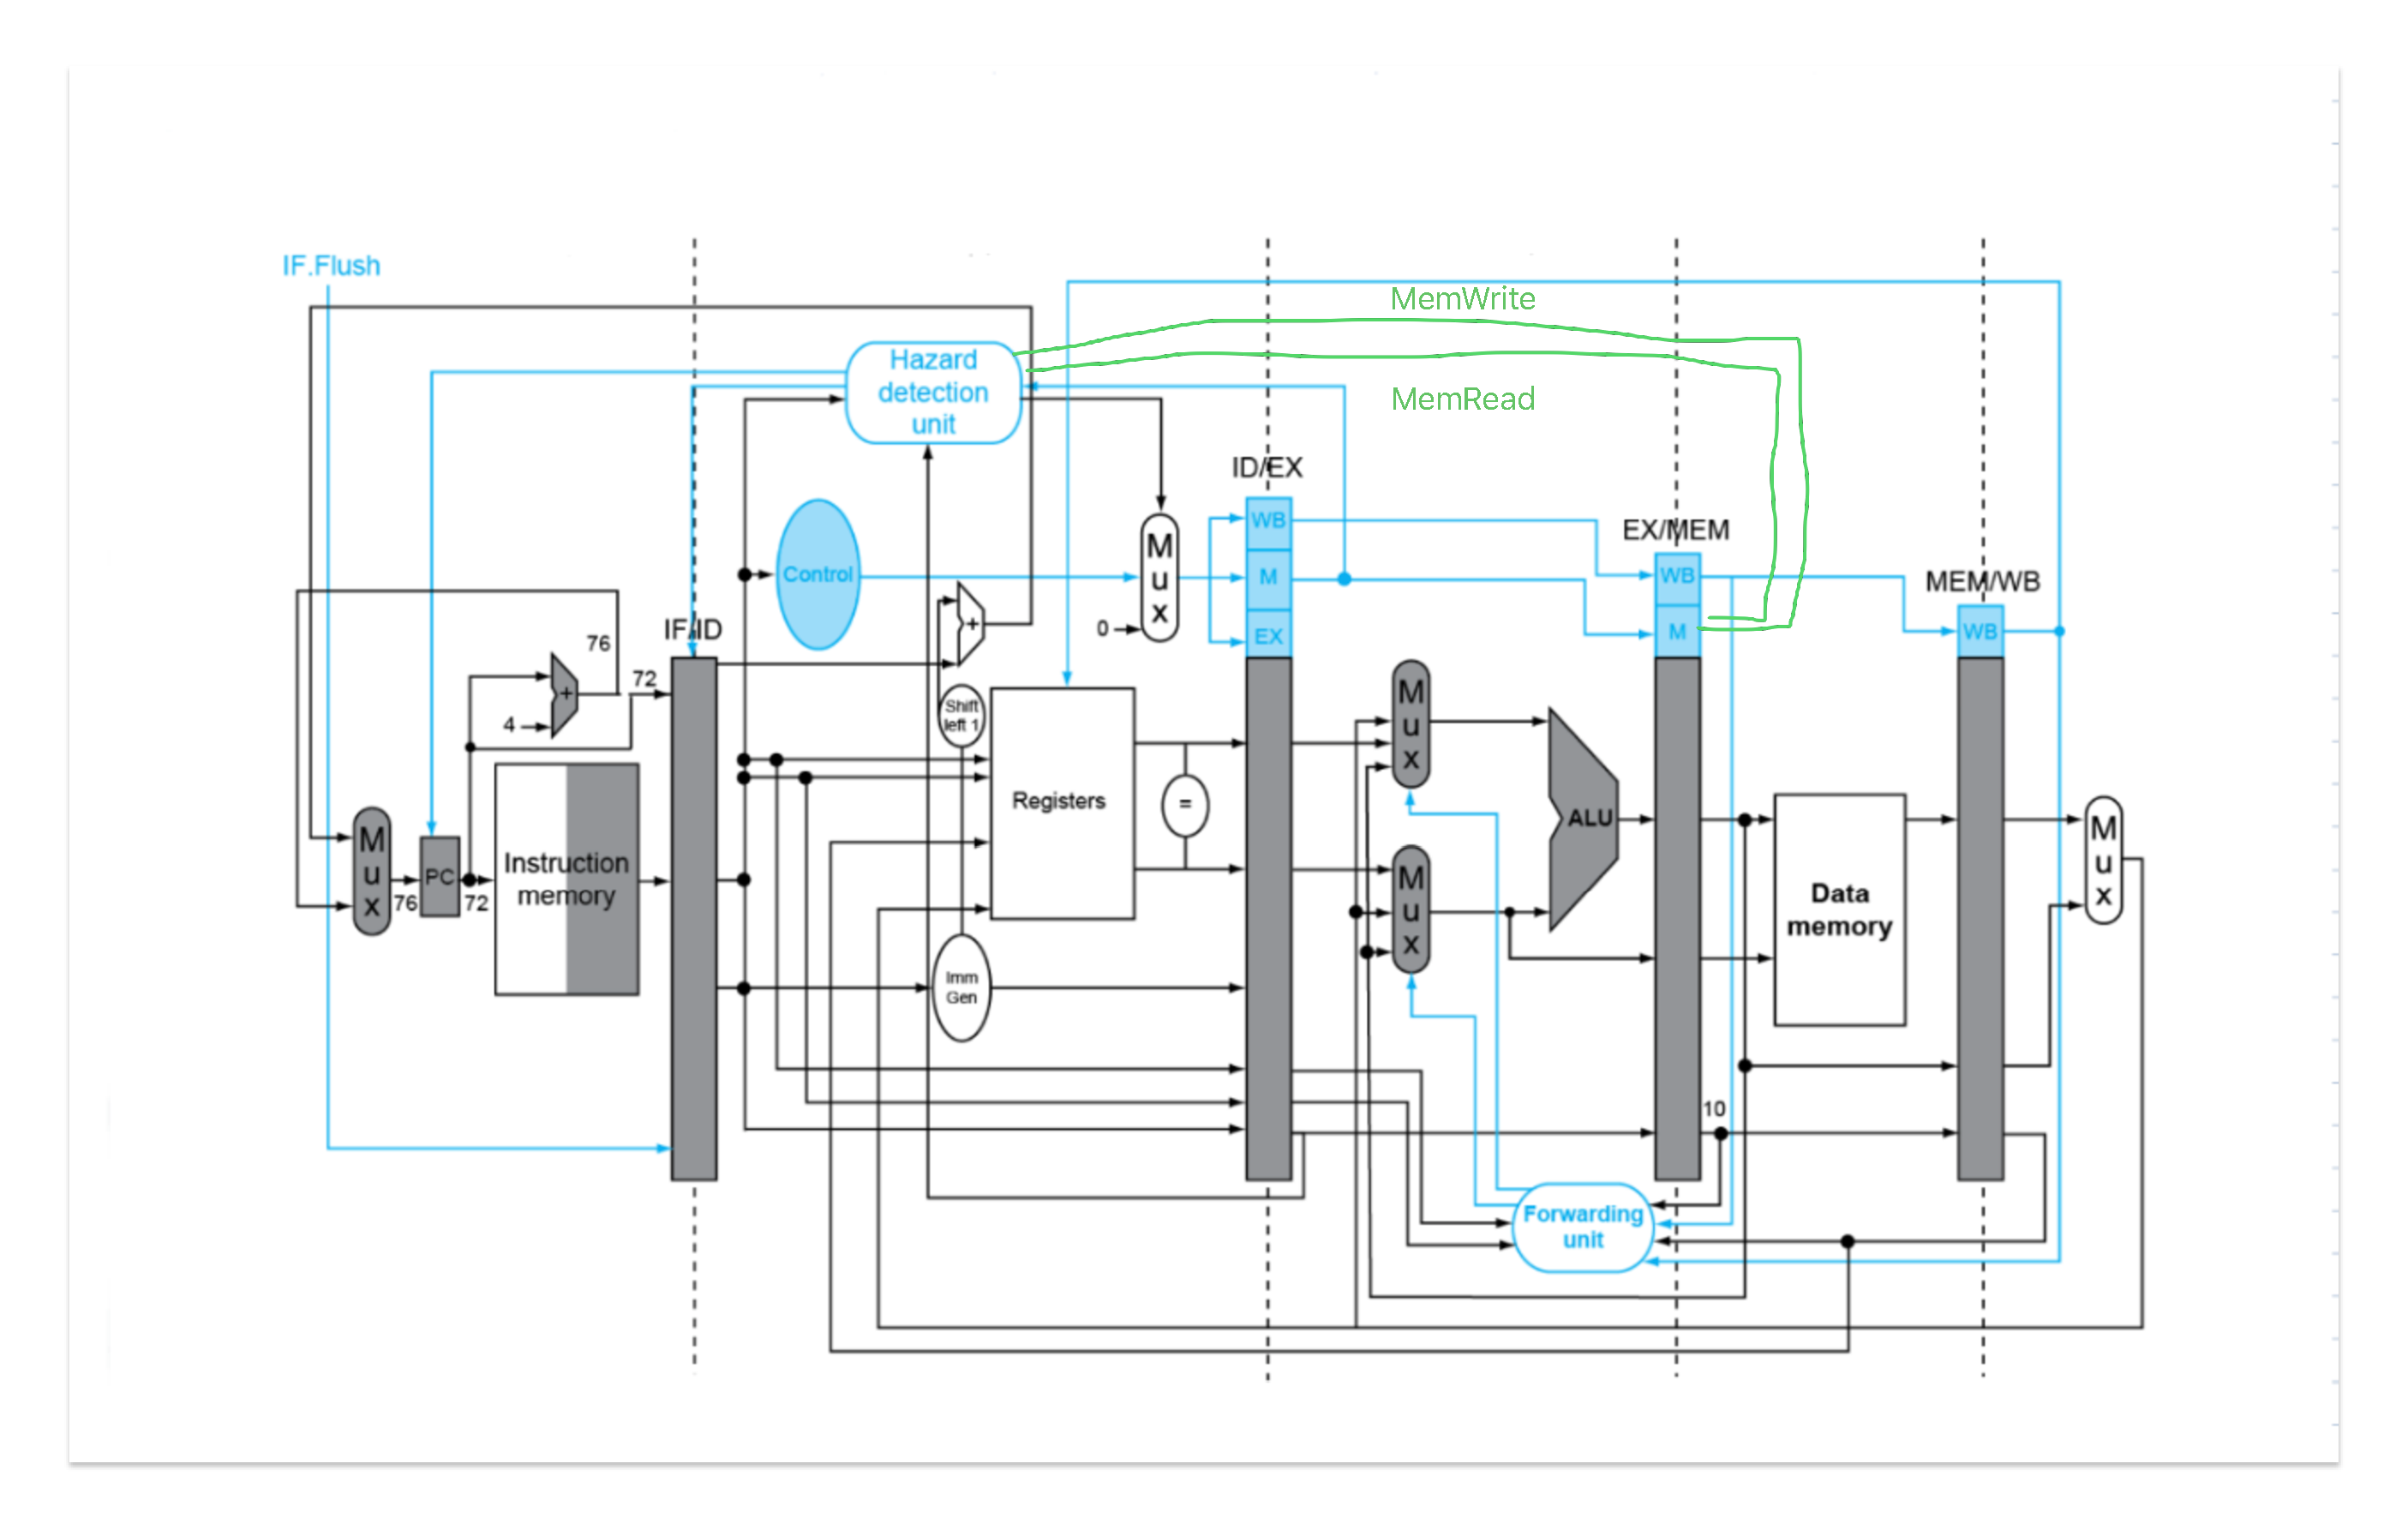
\includegraphics[width=.89\linewidth]{struct_hazard}
\caption{}
\label{fig:struct}
\end{figure}

\subsection{Tables}

\begin{table}[hbp]
\caption{If memory could not read and write simultaneously}
\label{tab:struct}
\centering
%\begin{tabular}{cccccccc}
%Cycle & \texttt{sd} & \texttt{ld x31} & \texttt{ld x28} & \texttt{add} & \texttt{beq} & \texttt{and} & \texttt{or} \\
%\hline
%1 & \texttt{IF} \\
%2 & \texttt{ID} & \texttt{IF} \\
%3 & \texttt{EX} & \texttt{ID} & \texttt{IF} \\
%4 & \texttt{MEM} & \texttt{EX} & \texttt{ID} & stall \\
%5 & \texttt{WB} & \texttt{MEM} & \texttt{EX} & stall \\
%6 &             & \texttt{WB} & \texttt{MEM} & stall \\
%7 &             &             & \texttt{WB} & \texttt{IF} \\
%8 &             &             &             & \texttt{ID} & \texttt{IF} \\
%9 &             &             &             & \texttt{EX} & \texttt{ID} & \texttt{IF} \\
%10 &             &             &             & \texttt{MEM} & \texttt{EX} & \texttt{ID} & \texttt{IF} \\
%11 &             &             &             & \texttt{WB} & \texttt{MEM} & \texttt{EX} & \texttt{ID} \\
%12 &             &             &             &             & \texttt{WB} & \texttt{MEM} & \texttt{EX} \\
%13 &             &             &             &             &             & \texttt{WB} & \texttt{MEM} \\
%14 &             &             &             &             &             &             & \texttt{WB}
\begin{tabular}{ccccccccccccccc}
Cycle & 1 & 2 & 3 & 4 & 5 & 6 & 7 & 8 & 9 & 10 & 11 & 12 & 13 & 14 \\
\hline
\texttt{sd} & \texttt{IF} & \texttt{ID} & \texttt{EX} & \texttt{MEM} & \texttt{WB} \\
\texttt{ld x31} && \texttt{IF} & \texttt{ID} & \texttt{EX} & \texttt{MEM} & \texttt{WB}\\
\texttt{ld x28} &&& \texttt{IF} & \texttt{ID} & \texttt{EX} & \texttt{MEM} & \texttt{WB}\\
\texttt{add} &&&& stall & stall & stall & \texttt{IF} & \texttt{ID} & \texttt{EX} & \texttt{MEM} & \texttt{WB} \\
\texttt{beq} &&&&&&&& \texttt{IF}& \texttt{ID} & \texttt{EX} & \texttt{MEM} & \texttt{WB} \\
\texttt{and} &&&&&&&&& \texttt{IF} & \texttt{ID} & \texttt{EX} & \texttt{MEM} & \texttt{WB} \\
\texttt{or} &&&&&&&&&& \texttt{IF} & \texttt{ID} & \texttt{EX} & \texttt{MEM} & \texttt{WB}
\end{tabular}
\end{table}

\begin{table}[hbp]
\caption{If memory could read and write simultaneously}
\label{tab:struct_simultaneous}
\centering
\begin{tabular}{cccccccccccccc}
Cycle & 1 & 2 & 3 & 4 & 5 & 6 & 7 & 8 & 9 & 10 & 11 & 12 & 13 \\
\hline
\texttt{sd} & \texttt{IF} & \texttt{ID} & \texttt{EX} & \texttt{MEM} & \texttt{WB} \\
\texttt{ld x31} && \texttt{IF} & \texttt{ID} & \texttt{EX} & \texttt{MEM} & \texttt{WB}\\
\texttt{ld x28} &&& \texttt{IF} & \texttt{ID} & \texttt{EX} & \texttt{MEM} & \texttt{WB}\\
\texttt{add} &&&& \texttt{IF} & \texttt{ID} & \texttt{EX} & \texttt{MEM} & \texttt{WB} \\
\texttt{beq} &&&&& stall & stall & \texttt{IF}& \texttt{ID} & \texttt{EX} & \texttt{MEM} & \texttt{WB} \\
\texttt{and} &&&&&&&& \texttt{IF} & \texttt{ID} & \texttt{EX} & \texttt{MEM} & \texttt{WB} \\
\texttt{or} &&&&&&&&& \texttt{IF} & \texttt{ID} & \texttt{EX} & \texttt{MEM} & \texttt{WB}
\end{tabular}
\end{table}

\section{Data Hazard}

\subsection{Neither Forwarding Unit Nor Hazards Detection}

We should insert 2 bubbles between the second \texttt{ld} and the first \texttt{add}, and another 2 bubbles between the first and the second \texttt{add}.

\subsection{Only Forwarding Unit But No Hazards Detection}

We should insert a bubble between the second \texttt{ld} and the first \texttt{add}.

\subsection{Both Forwarding Unit And Hazards Detection}

\subsubsection{Stall on Load-Use Hazard}

We would detect the hazard and stall when the second \texttt{ld} is in the \texttt{EX} stage, which occurred in cycle 4.

\subsubsection{\texttt{EX}/\texttt{MEM} Forward}

We would forward from when \texttt{EX}/\texttt{MEM} pipeline register to one of the input of ALU when the second \texttt{add} is in the \texttt{EX} stage, which occurred in cycle 7.

\subsubsection{\texttt{MEM}/\texttt{WB} Forward}

We would forward from when \texttt{MEM}/\texttt{WB} pipeline register to one of the input of ALU when the first \texttt{add} is in the \texttt{EX} stage, which occurred in cycle 6.

\subsection{Both Forwarding Unit And Hazards Detection (cont.)}

There are 4 instructions and we have to insert a \texttt{nop}, so in total it takes $5+(4+1)-1=9$ cycles.

\section{Pipeline Performance}

The cycle time is $\frac{10^9}{300\times10^6}=\frac{10}{3}$ns.

\subsection{7-stage Pipeline}

$S=30\times\frac{3}{10}-7+1=3$, thus
$$30+4\times3\times\frac{10}{3}=70$$

\subsection{$N$-stage Pipeline}

$$\left\{\begin{array}{rrr}
N+&(S-1)=&90\times\frac{3}{10}=27\\
N+&(6S-1)=&290\times\frac{3}{10}=87\\
\end{array}\right.$$, so we have $S=12,N=16$.

\section{Branch Prediction}

\subsection{Always-Taken \& Alway-Not-Taken}

The accuracy rate:
\begin{description}
\item[Always-Taken] $\frac{3}{8}=37.5\%$
\item[Always-Not-Taken] $\frac{5}{8}=62.5\%$
\end{description}

\subsection{1-bit Dynamic}

\begin{table}[htp]
\caption{1-bit Dynamic Predictor}
\label{tab:1bit}
\centering
\begin{tabular}{ccc}
Predict & Outcome & Correct \\
\hline
T & T & \checkmark \\
T & NT & \\
NT & NT & \checkmark \\
NT & NT & \checkmark \\
NT & NT & \checkmark \\
NT & T & \\
T & NT & \\
NT & T & \\
\end{tabular}
\end{table}

The accuracy rate is $\frac{4}{8}=50\%$.

\subsection{2-bit Dynamic}

\begin{table}[H]
\caption{2-bit Dynamic Predictor}
\label{tab:2bit}
\centering
\begin{tabular}{ccc}
State & Outcome & Correct \\
\hline
Strongly Not Taken & T & \\
Weakly Not Taken & NT & \checkmark \\
Strongly Not Taken & NT & \checkmark \\
Strongly Not Taken & NT & \checkmark \\
Strongly Not Taken & NT & \checkmark \\
Strongly Not Taken & T & \\
Weakly Not Taken & NT & \checkmark \\
Strongly Not Taken & T &  \\
\end{tabular}
\end{table}

The accuracy rate is $\frac{5}{8}=62.5\%$.

\section{Exception with Pipeline}

\begin{table}[htp]
\caption{}
\label{tab:exceptions}
\centering
\renewcommand{\arraystretch}{1.5}
\begin{tabular}{cccccc}
Cycle & \texttt{IF} & \texttt{ID} & \texttt{EX} & \texttt{MEM} & \texttt{WB} \\
\hline
1 & \texttt{ld} \\
2 & \texttt{sub} & \texttt{ld} \\
3 & \texttt{beq} & \texttt{sub} & \texttt{ld} \\
4 & \texttt{beq} & \texttt{sub} & bubble & \texttt{ld} \\
5 & \texttt{sd} & \texttt{beq} & \texttt{sub} & bubble & \texttt{ld} \\
6 & \makecell{1\textsuperscript{st} instruction of \\ exception handler} & bubble & bubble & \texttt{sub} & bubble \\
\end{tabular}
\end{table}

\end{document}
